\documentclass{article}
\usepackage{xcolor}
\definecolor{cit}{RGB}{0,0,255}  % Define 'cit' as blue
\usepackage{color}
\usepackage{amsmath,amsfonts,amssymb,bm}
\usepackage{natbib}
\bibliographystyle{plainnat}
\usepackage{hyperref}
\usepackage{graphicx}

% Custom commands
\newcommand{\diag}{\operatorname{diag}}
\newcommand{\innp}[1]{\left\langle #1 \right\rangle}
\newcommand{\bdot}[1]{\mathbf{\dot{ #1 }}}
\newcommand{\OPT}{\operatorname{OPT}}
\newcommand{\mA}{\mathbf{A}}
\newcommand{\mP}{\mathbf{P}}
\newcommand{\mLambda}{\mathbf{\Lambda}}
\newcommand{\ones}{\mathds{1}}
\newcommand{\zeros}{\textbf{0}}
\newcommand{\vx}{\mathbf{x}}
\newcommand{\vp}{\mathbf{p}}
\newcommand{\vn}{\mathbf{n}}
\newcommand{\dd}{\mathrm{d}}
\newcommand{\cx}{\mathcal{X}}
\newcommand{\cy}{\mathcal{Y}}
\newcommand{\cc}{\mathcal{C}}
\newcommand{\cz}{\mathcal{Z}}
\newcommand{\vxh}{\mathbf{\hat{x}}}
\newcommand{\vyh}{\mathbf{\hat{y}}}
\newcommand{\vzh}{\mathbf{\hat{z}}}
\newcommand{\vy}{\mathbf{y}}
\newcommand{\vz}{\mathbf{z}}
\newcommand{\vv}{\mathbf{v}}
\newcommand{\ve}{\mathbf{e}}
\newcommand{\va}{\mathbf{a}}
\newcommand{\vw}{\mathbf{w}}
\newcommand{\vsigma}{\bm{\sigma}}
\newcommand{\vvh}{\mathbf{\hat{v}}}
\newcommand{\vb}{\mathbf{b}}
\newcommand{\vg}{\mathbf{g}}
\newcommand{\vu}{\mathbf{u}}
\newcommand{\vub}{\overline{\mathbf{u}}}
\newcommand{\vuh}{\hat{\mathbf{u}}}
\newcommand{\veta}{\bm{\eta}}
\newcommand{\vetah}{\bm{\hat{\eta}}}
\newcommand{\defeq}{\stackrel{\mathrm{\scriptscriptstyle def}}{=}}
\newcommand{\etal}{\textit{et al}.}
\newcommand{\tnabla}{\widetilde{\nabla}}
\newcommand{\tE}{\widetilde{E}}
\newcommand{\rr}{\mathbb{R}}
\newcommand{\norm}[1]{\left\lVert#1\right\rVert}
\newcommand{\bmat}[1]{\begin{bmatrix}#1\end{bmatrix}} 
\newcommand{\inner}[2]{\langle#1,#2\rangle}
\newcommand{\ri}{\mathbf{r}_i}
\newcommand{\rj}{\mathbf{r}_j}
\newcommand{\rij}{\mathbf{r}_{ij}}
\newcommand{\grad}{\nabla}
\newcommand{\Hess}{\nabla\nabla}
\usepackage{enumitem}

\begin{document}

\begin{center}
    \LARGE Smoothed Particle Hydrodynamics and its applications in Lunar Rover Simulation
\end{center}

\begin{center}
    \large Continuum Modelling, Multi-resolution and Consistency related aspects
\end{center}

\begin{center}
    \large Huzaifa Mustafa Unjhawala
\end{center}

\begin{center}
    \large Dec 11, 2024
\end{center}


\section{Introduction}
This summary report discusses the Smoothed Particle Hydrodynamics (SPH) method, a popular method to solve PDE's and its applications in Lunar Rover Simulation. Due to scope of the document, the content is focussed on three interesting components: 

\begin{enumerate}
    \item Continuum Modelling of the Lunar Soil.
    \item Use of Multi-resoultion to save computational cost.
    \item Ways in which consistency of the SPH method is improved.
\end{enumerate}
In addition to these components, Smoothed Particle Hydrodynamics is introduced and some aspects of handling of Boundary Conditions is discussed. These introductions provide the reader with sufficient context to understand the interesting components of the project.  

The report is structured as follows; first a motivation for the project is provided. This is followed by a discussion on the SPH method and the handling of Boundary Conditions. Then the continuum modelling of the Lunar Soil is discussed. This is followed by a discussion on the use of Multi-resolution to save computational cost. Finally, the ways in which consistency of the SPH method is improved are discussed.

\section{Motivation}
Lunar Rover Simulation is a complex problem as it requires the modelling of the rover - which is a multi-body system with multiple degrees of freedom and constraints (the joints holding the rover together), the interaction of the rover with the lunar surface -- which is a granular material. In this document the focus is mostly on the interaction of the rover with the lunar surface. To model the lunar surface, a popular approach is the Discrete Element Method (DEM)~\citep{zhang2023gpu} where each grain is represented by a sphere and the interactions between the grains are modelled using contact mechanics. This method is however computationally expensive as the size of each grain is usually in the order of microns resulting in tens of millions of grains to model the lunar surface~\citep{carrier1973lunar}. The approach discussed herein models the Lunar surface as a continuum, drastically reducing the degrees of freedom and the computational cost. The methodology chosen to discretize the continuum is Smoothed Particle Hydrodynamics (SPH)~\citep{monaghan1992smoothed}.

\section{Smoothed Particle Hydrodynamics}
Smoothed Particle Hydrodynamics is computational method to solve PDE's. The computational domain of interest is discretized using a set of particles. The particles are then used to approximate the properties of the continuum such as density, pressure, velocity, etc. The SPH method is thus a Lagrangian, mesh free method.  

The basic principle of SPH is to approximate the value of a function and its gradient based on the spatial weighted average of the neighboring particles. 
\subsection*{Function Approximation}
Consider a scalar function (can be extended to vector functions) of interest $f(\vx)$. Using the Dirac delta function, the value of the function at a point $\vx$ is given by:
\begin{equation}
  \label{eq:diracDeltaIdentity}
  f(\vx) = \int_\Omega f(\vx') \delta(\vx - \vx') \dd{\vx'}.
\end{equation}
Where $\delta(\vx - \vx')$ is the Dirac Delta function given by:
\begin{equation}
  \delta(\vx - \vx') = \begin{cases}
      1 & \vx = \vx' \\
      0, & \vx \neq \vx'
  \end{cases}
\end{equation}
Note, $\Omega$ is the volume of the integral that contains $\vx$. Eq.~\ref{eq:diracDeltaIdentity} is exact with no approximations, provided $f(\vx')$ is defined and continuous in $\Omega$. 
The SPH method then makes what is so called the \textit{kernel approximation} to Eq.~\ref{eq:diracDeltaIdentity} where the impossible to numerically compute Dirac Delta function is replaced with a smoothing function, popularly called the \textit{kernel function} or \textit{smoothing kernel}. Making this change gives us the \textit{kernel approximation} of $f(\vx)$ as:
\begin{equation}
    \label{eq:kernelApproximation}
    \langle f(\vx) \rangle = \int_\Omega f(\vx') W(\vx - \vx', h) \dd{\vx'}.
\end{equation}
Where $W(\vx - \vx', h)$ is the smoothing kernel, $h$ is the smoothing length, and $\Omega$ is the volume of the integral that contains $\vx$. There are certain properties that the smoothing kernel must satisfy, see~\citep{liu2010sph} for more details.  
Next we make the particle approximation to the integral in Eq.~\ref{eq:kernelApproximation} by replacing the integral with a sum over all the particles over which the smoothing kernel has influence (given by $kh$). This gives us the following equation:
\begin{equation}
    \label{eq:particleApproximation}
    \langle f(\vx_i) \rangle = \sum_{j=1}^{N_i} V_j f(\vx_j) W(\vx_i - \vx_j, h).
\end{equation}
Where $N_i$ are the neighbors of particle $i$ and $V_j$ is the volume of the neighboring particle $j$. As you would imagine, the error due to the kernel approximation increases as the smoothing length $h$ increases whereas the error due to the particle approximation decreases as the number of particles in the neighborhood increases. The exact relationships for the error due to the kernel approximation and the particle approximation are left to~\citep{liu2010sph}.
\subsection*{Gradient Approximation}
Now, we move onto deriving the spatially discretized form of gradient of a scalar function (for vector function, same applies with the divergence operator) at an SPH marker. We start from Eq.~\ref{eq:kernelApproximation} replace $f(\vx)$ with $\nabla \cdot \mathbf{f}(\vx)$. This gives us the following equation:
\begin{equation}
    \label{eq:SimplekernelApproxSPHGradient}
    \langle \nabla f(\vx) \rangle = \int_\Omega \left[ \nabla f(\vx') \right] W(\vx - \vx', h) \dd{\vx'}.
\end{equation}
Using chain rule, we can rewrite the RHS of the above equation as:
\begin{equation}
    \int_\Omega \left[ \nabla f(\vx') \right] W(\vx - \vx', h) \dd{\vx'} = \int_\Omega \left[ \nabla \left( f(\vx') W(\vx - \vx', h) \right) - f(\vx') \nabla W(\vx - \vx', h) \right] \dd{\vx'}.
\end{equation}
Applying the divergence theorem to the first term, we get:
\begin{equation}
    \int_{S} f(\vx') W(\vx - \vx', h)\vn \dd{S}.
\end{equation}
Since the kernel is compact support, the kernel value will evaluate to zero at the boundaries of the kernel support. Thus, the first term vanishes and we are left with:
\begin{equation}
    \label{eq:kernelApproxSPHGradient}
    \langle \nabla f(\vx) \rangle = \int_\Omega - f(\vx') \nabla W(\vx - \vx', h) \dd{\vx'}.
\end{equation}
Making the particle approximation, we get:
\begin{equation}
    \label{eq:kernelApproxSPHGradientParticles}
    \langle \nabla f(\vx_i) \rangle = - \sum_{j=1}^{N_i} V_j f(\vx_j) \nabla_j W(\vx_i - \vx_j, h).
\end{equation}
Since the kernel is an even function, the gradient of the kernel is an odd function. Using this, we can eliminate the negative sign in Eq.~\ref{eq:kernelApproxSPHGradientParticles}:
\begin{equation}
    \label{eq:kernelApproxSPHGradientParticlesPositive}
    \langle \nabla f(\vx_i) \rangle = \sum_{j=1}^{N_i} V_j f(\vx_j) \nabla_i W(\vx_i - \vx_j, h).
\end{equation}
\subsection*{Discretizing the Continuity equation}
Now, we use the concepts of the function approximation and gradient approximation to discretize the continuity equation which is given by:
\begin{equation}
  \label{eq:ContinuityEquation}
    \frac{\dd \rho}{\dd t} = - \rho \nabla \cdot \mathbf{v}.
\end{equation}
Thus, we need to discretize $\nabla \cdot \mathbf{v}$ with SPH. Observe using chain rule and using a general $f(\vx)$ as a field variable, we can write:
\begin{equation}
  \label{eq:GradientSPHContinuity}
  \nabla f|_i = \left. \frac{\nabla(\rho f) - f\nabla \rho}{\rho}\right|_i
\end{equation}
We can replace each of the gradient terms in the above equation with the SPH gradient operator given by Eq.~\ref{eq:kernelApproxSPHGradientParticles} (without the negative sign). Applying this to $\nabla(\rho f)$, we get:
\begin{equation}
  \label{eq:continuityTerm1}
  \nabla(\rho f)|_i = \sum_{j=1}^{N_i} V_j \left( \rho_j f_j \nabla_i W(\vx_i - \vx_j, h) \right).
\end{equation}
Similarly, applying Eq.~\ref{eq:kernelApproxSPHGradientParticles} to $\nabla \rho$, we get:
\begin{equation}
  \label{eq:continuityTerm2}
  \nabla \rho|_i = \sum_{j=1}^{N_i} V_j \left( \rho_j \nabla_i W(\vx_i - \vx_j, h) \right).
\end{equation}
Substituting these into Eq.~\ref{eq:GradientSPHContinuity}, we get:
\begin{align}
  \nabla f|_i &= \sum_{j=1}^{N_i} V_j \left( \frac{\rho_j f_j \nabla_i W(\vx_i - \vx_j, h) - f_i \rho_j \nabla_i W(\vx_i - \vx_j, h)}{\rho_i} \right). \\
  \nabla f|_i &= \frac{1}{\rho_i} \sum_{j=1}^{N_i} V_j \left( \rho_j f_j \nabla_i W(\vx_i - \vx_j, h) - f_i \rho_j \nabla_i W(\vx_i - \vx_j, h) \right).
\end{align}
Usually, $V_j$ is taken as $m_j / \rho_j$ where $m_j$ is the mass of the particle $j$. This gives:
\begin{equation}
  \label{eq:contGradientOp}
  \nabla f|_i = \frac{1}{\rho_i} \sum_{j=1}^{N_i}  m_j \left( f_j - f_i \right) \nabla_i W(\vx_i - \vx_j, h).
\end{equation}
In the continuity equation, $f = \vv$. Thus we get:
\begin{equation}
  \nabla \cdot \vv|_i = \frac{1}{\rho_i} \sum_{j=1}^{N_i}  m_j \left( \vv_j - \vv_i \right) \cdot \nabla_i W(\vx_i - \vx_j, h).
\end{equation}
Putting this back into Eq.~\ref{eq:ContinuityEquation}, we get:
\begin{equation}
  \frac{\dd \rho}{\dd t} = - \rho \nabla \cdot \vv = - \sum_{j=1}^{N_i}  m_j \left( \vv_j - \vv_i \right) \cdot \nabla_i W(\vx_i - \vx_j, h).
\end{equation}
\subsection*{Discretizing the Momentum Equation}
Using a similar approach, we can discretize the momentum equation which is given by:
\begin{equation}
  \label{eq:MomentumEquation}
  \frac{\dd \vv}{\dd t}  = \frac{1}{\rho} \nabla \cdot \vsigma + \mathbf{f_{ext}}.
\end{equation}
This time however we use a different spatial differential operator in order to conserve Linear and Angular Momentum. In Sec.~\ref{sec:consistency} we discuss the trade-off in consistency that we need to pay to conserve linear and angular momentum. The differential operator is derived by starting with the following version of the chain rule:
\begin{equation}
  \label{eq:chainRule2}
  \nabla f|_i = \left. \rho \left[\nabla \left( \frac{f}{\rho} \right) + \frac{f}{\rho^2}\nabla \rho \right]\right|_i
\end{equation}
Again, we will proceed by applying the gradient operator given by Eq.~\ref{eq:kernelApproxSPHGradientParticles} to each of the terms with a gradient in the above equation. For term $\nabla \left( \frac{f}{\rho} \right)$, we get:
\begin{equation}
  \label{eq:momentumTerm1}
  \nabla \left. \left( \frac{f}{\rho} \right)\right|_i = \sum_{j=1}^{N_i} V_j \left( \frac{f_j}{\rho_j} \nabla_i W(\vx_i - \vx_j, h) \right).
\end{equation}
Then, for term $\nabla \rho$, we get:
\begin{equation}
  \label{eq:momentumTerm2}
  \nabla \rho|_i = \sum_{j=1}^{N_i} V_j \left( \rho_j \nabla_i W(\vx_i - \vx_j, h) \right).
\end{equation}
Substituting these into Eq.~\ref{eq:chainRule2}, we get:
\begin{equation}
  \nabla f|_i =  \rho_i \left[\sum_{j=1}^{N_i} V_j \left( \frac{f_j}{\rho_j} \nabla_i W(\vx_i - \vx_j, h) \right) + \frac{f_i}{\rho_i^2} \sum_{j=1}^{N_i} V_j \left( \rho_j \nabla_i W(\vx_i - \vx_j, h) \right) \right]
\end{equation}
Using $V_j = m_j / \rho_j$, we get:
\begin{equation}
  \nabla f|_i =  \rho_i \left[\sum_{j=1}^{N_i} m_j \left( \frac{f_j}{\rho_j^2} \nabla_i W(\vx_i - \vx_j, h) \right) + \frac{f_i}{\rho_i^2} \sum_{j=1}^{N_i} m_j \left(\nabla_i W(\vx_i - \vx_j, h) \right) \right].
\end{equation}
Taking common terms out, we get:
\begin{equation}
  \nabla f|_i =  \rho_i \left[\sum_{j=1}^{N_i} m_j \left[ \frac{f_j}{\rho_j^2} + \frac{f_i}{\rho_i^2} \right] \nabla_i W(\vx_i - \vx_j, h) \right].
\end{equation}
In the momentum equation, we have $f = \vsigma$. Thus we get:
\begin{equation}
  \nabla \cdot \vsigma|_i =  \rho_i \left[\sum_{j=1}^{N_i} m_j \left[ \frac{\vsigma_j}{\rho_j^2} + \frac{\vsigma_i}{\rho_i^2} \right] \cdot \nabla_i W(\vx_i - \vx_j, h) \right].
\end{equation}
Thus, the momentum equation becomes:
\begin{equation}
  \label{eq:momentumEquationSPHDiscretized}
  \left. \frac{\dd \vv}{\dd t}\right|_i = \rho_i \left[\sum_{j=1}^{N_i} m_j \left[ \frac{\vsigma_j}{\rho_j^2} + \frac{\vsigma_i}{\rho_i^2} \right] \cdot \nabla_i W(\vx_i - \vx_j, h) \right] + \mathbf{f_{ext}}|_i.
\end{equation}
\subsection*{Boundary Conditions}
Lunar Rover simulations require more than just modelling the Lunar terrain. The rover also needs to interact with the lunar surface. This interaction is modelled using a ``co-simulation'' framework. Here, the parts of the rover is modelled as a rigid body and its dynamics are computed with a separate rigid body dynamics solver. Thus, from the terrain's perspective, the rigid bodies just move through the terrain at each time step. However, we still need to model the interaction between these rigid bodies and the terrain i.e. we need to ensure that the terrain does not penetrate the rigid bodies. Additionally, we would also like to model the ``friction'' between the rover and the lunar surface. For this we leverage the Adami Boundary Conditions introduced in~\citep{adami2012generalized}. The power of Adami BC's comes because they can handle arbitrarily shaped boundary conditions in two and three dimensions. This is done by discretizing the solid boundaries with \textit{dummy particles} (which we call \textit{Boundary Condition Enforcing} (BCE) markers). Dummy particles ensure that the support of the kernel interpolants is fully contained within the fluid phase. The pressure and shear stress at a wall particle position for the force calculation is calculated from the surrounding fluid particles with a boundary condition. Including the solid particles in the density change rate calculation ensures a pressure response when fluid particles approach a wall, i.e. the impermeability condition of solid walls is fulfilled. It is important to note however that these BCE markers do not move according to SPH dynamics. Rather they are moved using the rigid body dynamics solver. Their sole purpose is thus just to ``trick'' the SPH particles and incorporate the boundary conditions of interest.
\subsubsection*{No-Slip Boundary Conditions}
To implement a no slip BC, first, the velocity at a BCE marker is extrapolated from the fluid markers as
$$\tilde{v}_a = \frac{\sum_b v_b w_{ab}}{\sum_b w_{ab}}$$
Here, $b$ corresponds to all fluid markers and $W_{ab}$ is the kernel function evaluation between BCE marker $a$ and fluid marker $b$.  
Then, to impose a no-slip boundary condition, the BCE markers are given a velocity of
$$v_w = 2v_a - \tilde{v}_a$$, where $v_a$ is the wall prescribed velocity. $v_a = 0$ for fixed boundaries and for rigid boundaries, we get $v_a$ from the Chrono dynamics solver through the FSI interface.
\begin{figure}[h]
  \centering
  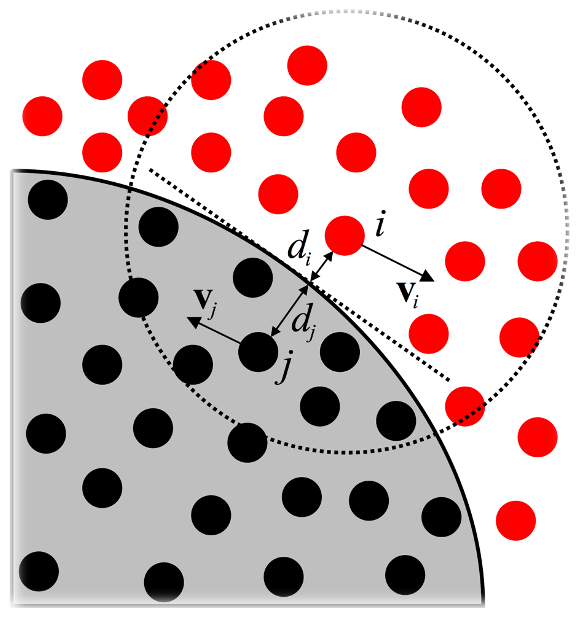
\includegraphics[width=0.25\textwidth]{./img/bc.png}
  \caption{Herein we see how the velocity is extrapolated from the fluid markers (Red) to the BCE markers (Black). The BCE markers are then given a velocity of $v_w = 2v_a - \tilde{v}_a$ to enforce the no-slip BC.}
  \label{fig:noSlipBC}
\end{figure}
\subsubsection*{Stress Boundary Conditions to prevent penetration}
In a similar vein, the stress at each BCE marker is extrapolated from the fluid markers as~\citep{StressBC}:
$$\sigma_s^{ij} = \frac{\sum_f \sigma_f^{ij} W(x_{sf}) \left( g^i - a_s^i \right) - \sum_f p_f^i W(x_{sf}) \delta^{ij}}{\sum_f W(x_{sf})}
$$
\section{Continuum Modelling of the Lunar Soil}
Now we reach the stage where we must make a choice of what we intended to simulate with this machinery. This is equivalent to choosing the equations for the stress $\sigma$ in the momentum equation~\ref{eq:MomentumEquation}. The choice of equations for $\sigma$ is equivalent to choosing the constitutive model for the soil. The stress tensor is usually expressed as:
\begin{equation}\label{equ:stress_tensor}
  \boldsymbol{\sigma} =-p{\bf I}+\boldsymbol{\tau},
\end{equation}
where $p$ is the isotropic pressure and $\boldsymbol{\tau}$ is the deviatoric component of the stress tensor. The isotropic pressure is defined as the trace of the stress tensor, i.e.,  $p=-\frac{1}{3}\mathrm{tr}(\boldsymbol{\sigma}) = -\frac{1}{3}(\sigma_{xx}+\sigma_{yy}+\sigma_{zz})$. According to Hooke's law, a linear elastic relation between the Jaumann stress rate tensor and elastic strain tensors can be used to obtain the stress rate tensor as 
%
\begin{equation}\label{equ:stress_rate}
\frac{d\boldsymbol{\sigma}}{dt} = \dot{\boldsymbol{\phi }}\cdot{\boldsymbol{\sigma}}-{\boldsymbol{\sigma}}\cdot\dot{\boldsymbol{\phi }} + \overset{\triangle}{\boldsymbol{\sigma}},
\end{equation}
here the rotation rate tensor is defined as $\dot{\boldsymbol{\phi }} =\frac{1}{2}(\nabla\textbf{u} - \nabla\textbf{u}^\intercal)$, the Jaumann rate of the stress tensor is expressed as
%
\begin{equation}\label{equ:jaumann}
	\overset{\triangle}{\boldsymbol{\sigma}} =  2G(\dot{\boldsymbol{\varepsilon}}-\frac{1}{3}\mathrm{tr}(\dot{\boldsymbol{\varepsilon}}){\bf I}) + \frac{1}{3}K\mathrm{tr}(\dot{\boldsymbol{\varepsilon}}){\bf I},
\end{equation}
%
and the elastic strain rate tensor is defined as  $\dot{\boldsymbol{\varepsilon}} =\frac{1}{2}(\nabla\textbf{u} + \nabla\textbf{u}^\intercal)$ in the absence of plastic flow. Herein, $K$ denotes the bulk modulus of the material and satisfies $K=\frac{2(1+\nu)}{3(1-2\nu)}G$, where $G$ and $\nu$ are the shear modulus and Poisson’s ratio. Once the granular material starts to flow, the elastic strain rate tensor is defined as 
\[
\dot{\boldsymbol{\varepsilon}} =\frac{1}{2}(\nabla\textbf{u} + \nabla\textbf{u}^\intercal) - \frac{1}{\sqrt{2}}\dot{\lambda} \frac{\boldsymbol{\tau}}{\bar{\tau}} \; ,
\]
in which the second term comes from the contribution of the plastic flow of the granular material, and $\dot{\lambda}$ and $\bar{\tau}$ are the plastic strain rate and equivalent shear stress, respectively. Here we are required to define when the plastic flow starts. This is defined by the rheological model, and we use the one proposed by~\citep{Dunatunga2015}. A short motivation for why we require a yield criteria is best explained by Fig.~\ref{fig:yield_criteria}. Here we can see a simple hour-glass with a granular material. The granular material interestingly represents all three phases of the material, solid, liquid and gas. At the top of the hour glass, since the granular material is more packed together, it behaves like a solid. Futher down, closer to the hour glass, it behaves like a liquid and flows. As the granular material falls through the hole, it behaves like a gas where there is no tension amongst the individual grains. Thus, the rheology we choose, should, in some ways represent the granular material through its various phases.
\begin{figure}[h]
  \centering
  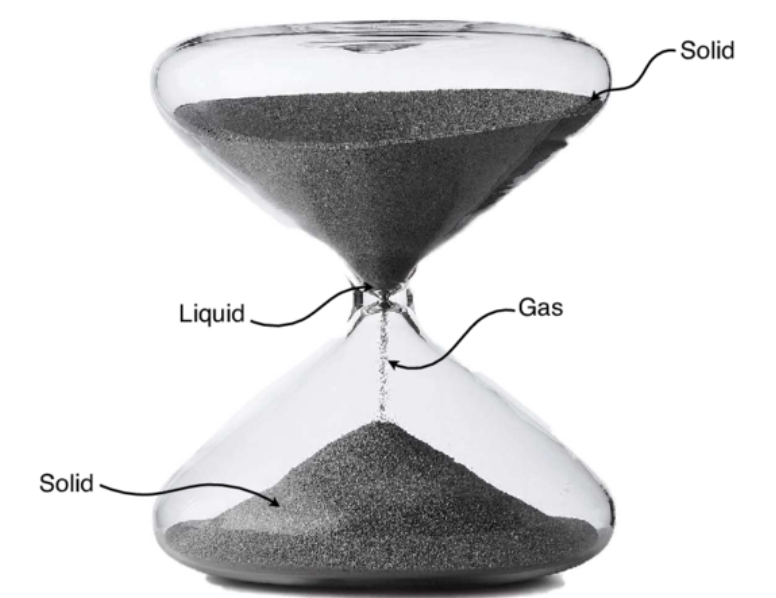
\includegraphics[width=0.25\textwidth]{./img/yield_criteria.png}
  \caption{Granular material in its three phases: solid, liquid and gas.}
  \label{fig:yield_criteria}
\end{figure}
\subsection*{Rheological Model}
We define the Drucker-Prager friction coefficient $\mu$ as $\mu =  \frac{\bar{\tau}}{p}$, where $p$ is the trace of the stress tensor $p = \frac{-1}{3}(\sigma_{xx}+\sigma_{yy}+\sigma_{zz})$ and $\bar{\tau}$ is the tensorial contraction (in simple terms, a scalar representing a matrix) of the deviatoric stress tensor  $\bar{\tau} = \sqrt{\frac{1}{2}\left(\tau : \tau\right)}$. Further, we define an inertial number $I$ that, given physical properties of the granular material, determines the ``friction'' of the material~\citep{Jop2006}. This relation is $I = \dot{\lambda} \frac{\sqrt{d^2\rho_s}}{\sqrt{p}}$. Here, $d$ is the mean particle size, $\rho_s$ is the density of the individual granular particles and $\dot{\lambda}$ is the plastic strain rate. Then, we define the friction coefficient as:
\begin{equation}
  \mu = \begin{cases} 
    \mu_s + \frac{\mu_2 - \mu_s}{\frac{I_0}{I} + 1}, & \text{if } I > 0 \\
    \mu \leq \mu_s, & \text{if } I = 0
  \end{cases}
\end{equation}
where $\mu$ is the angle of internal friction and $I_c$ is the critical inertial number.
Now, since $\mu$ is related to the stress through $\bar{\tau}$ and $p$, and $I$ is is related to the plastic strain rate $\dot{\lambda}$ the above is a closed rheological relation. We can thus rewrite this into a rate dependent form for the equivalent shear stress, given by:
\[
\bar{\tau} = \bar{\tau}(p, \dot{\lambda}) =
\begin{cases} 
    p \left( \mu_s + \frac{\mu_2 - \mu_s}{\xi \sqrt{p}/\dot{\lambda} + 1} \right), & \text{if } \dot{\gamma}^p > 0, \\
    \bar{\tau} \leq p\mu_s, & \text{if } \dot{\gamma}^p = 0
\end{cases}
\]
where $\xi = \frac{I_0}{\sqrt{d^2 \rho_s}}$. As we can see, this describes the yield between the solid and liquid phases of granular material. For liquid to gas, we define a critical density $\rho_c$ and set our stress to zero if the density of the particle is lesser than $\rho_c$:
\[\boldsymbol{\sigma} = 0 \text{ if } \rho < \rho_c.\]
Recall, all the equations here are in continuous form, both in space and time. In order to model this on a computer, they still need to be processed by the SPH machinery. In the interest of space, we will not go into these details here.
\section{Multi-resolution}
\subsection*{Motivation}
An important aspect of the SPH method is the spacing between the particles. From the principles of the method, one can intuitively see that the kernel support must always be filled with sufficient ``integration points''. This is especially true for the boundaries, where the boundaries must have the sufficient number of BCE markers to fill the kernel of the interacting fluid markers. Usually, this means that the solid bodies should have at least 3 layers of BCE markers (details left to ~\citep{adami2012generalized}). Additionally, the markers must be as uniformly distributed across the computation domain as possible (details left to~\citep{liu2010sph,adami2012generalized}). These two facts can pose a problem when we would like to simulate a thin solid structure with the granular material. Consider the wheel of the~\href{https://magazine.cs.cmu.edu/cmu-to-the-moon}{\textit{Moonranger}} rover that is to go to the moon in 2026 (Fig~\ref{fig:moonranger}).
\begin{figure}[h]
  \centering
  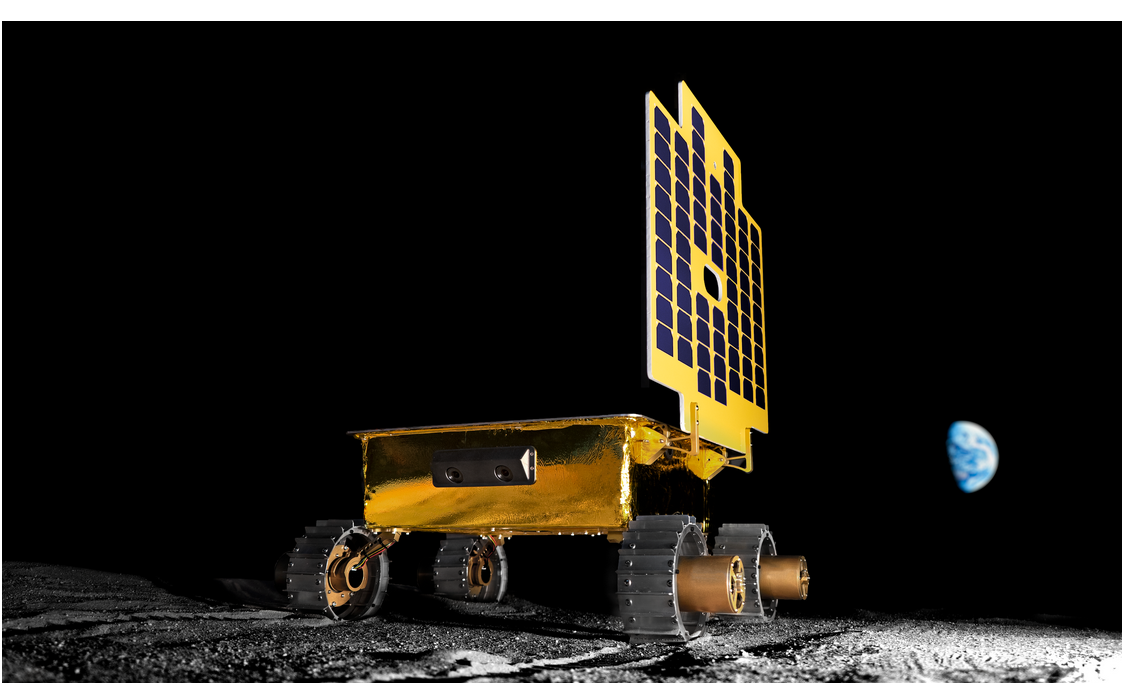
\includegraphics[width=0.5\textwidth]{./img/moonranger.png}
  \caption{The Moonranger rover developed by Carnegie Mellon University and simulated using SPH.}
  \label{fig:moonranger}
\end{figure}
This rover very small, about the size of a shoebox. Its wheels have grousers that are very thin, about $4$ mm thick (Fig.~\ref{fig:moonranger_wheel}). 
\begin{figure}[h]
  \centering
  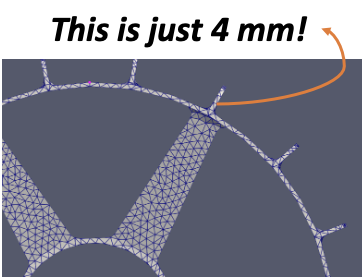
\includegraphics[width=0.3\textwidth]{./img/moonranger_wheel.png}
  \caption{The wheel of the~\href{https://magazine.cs.cmu.edu/cmu-to-the-moon}{\textit{Moonranger}} rover.}
  \label{fig:moonranger_wheel}
\end{figure}
To resolve this feature, we would require an SPH resolution of $2$ mm (to get three layers of BCE markers). With single-resolution, we would also have to resolve the Lunar granular material also with $2$ mm. If we are simulating $1$ m$^3$ of Lunar material, this would require $5 \times 10^6$ particles. This is a very large number of particles, and would require a lot of computational resources. This motivates the use of multi-resolution SPH which would allow us to resolve the thin solid features with a higher resolution than the granular material.
\subsection*{Implementation}
Thus, to allow for a different resolution for the solid body BCE markers, we start from Eq.~\ref{eq:kernelApproximation} and split the integral into two separate integrals, one over the region with only fluid and boundary markers and the other over the region with the solid body BCE markers. This gives us the following equation:
\begin{equation}
    \label{eq:multiResolutionSPH}
    \langle f(\vx) \rangle = \int_{\Omega_{fluid} \cup \Omega_{FB}} f(\vx') W(\vx - \vx', h) \dd{\vx'} + \int_{\Omega_{SB}} f(\vx') W(\vx - \vx', h) \dd{\vx'}.
\end{equation}
Where $\Omega_{fluid} \cup \Omega_{FB}$ is the sub volume which will be occupied by the fluid and fixed boundary markers (when the particle approximation is made) and $\Omega_{SB}$ is the sub volume which will be occupied by the solid body BCE markers.   

Then, making the particle approximation, we get:
\begin{equation}
    \label{eq:multiResolutionSPHParticles}
    \langle f(\vx_i) \rangle = \sum_{j=1}^{N_{fluid} \cup N_{FB}} V_j f(\vx_j) W(\vx_i - \vx_j, h) + \sum_{k=1}^{N_{SB}} V_k f(\vx_k) W(\vx_i - \vx_k, h_{SB}).
\end{equation}
Where $N_{fluid} \cup N_{FB}$ correspond to the neighbors of $i$ that are fluid of fixed boundary markers and $N_{SB}$ correspond to the neighbors of $i$ that are solid body markers. We make one assumption here:
\begin{enumerate}
    \item The smoothing length for the fluid, boundary and solid body markers are the same - This assumption will not lead to kernel truncation at the boundaries of the fluid and solid markers if and only if the solid BCE markers have a smaller volume than the fluid and boundary markers. Thus, for now we assume we always want to resolve the solid body markers at the same or finer resolution than the fluid and boundary markers.
\end{enumerate}
Thus, for multi-resolution SPH, each function value at an SPH marker is given by:
\begin{equation}
    \label{eq:multiResolutionSPHMarker}
    \langle f(\vx_i) \rangle = \sum_{j=1}^{N_{fluid} \cup N_{FB}} V_j f(\vx_j) W(\vx_i - \vx_j, h) + \sum_{k=1}^{N_{SB}} V_k f(\vx_k) W(\vx_i - \vx_k, h).
\end{equation}
This can further be extended to the gradient of the function and then further to the governing equations. In the interest of space, this is not detailed here. The new discretized equations would then allow us to resolve the thin solid features with a higher resolution than the granular material allowing for fewer particles and better computational performance.
\section{Consistency of the SPH method}
\label{sec:consistency}
Notice that while deriving the discretized form of the continuity and momentum equations we used different versions of the spatial gradient operator (Eq.~\ref{eq:chainRule2} and Eq.~\ref{eq:GradientSPHContinuity}). These choices directly affect the consistency of the SPH method which is defined as the maximum order of the polynomial that can be exactly reproduced by the method. In this case, we will focus on the gradient of a function and thus our definition of consistency becomes the maximum order of the polynomial that can be exactly reproduced by the gradient operator of SPH.
\subsection*{Consistency of gradient operator used in the continuity equation}
Rewriting Eq.~\ref{eq:contGradientOp} with $\omega = \frac{m}{\rho}$
\begin{equation}
    \label{eq:contGradientOp2}
    \nabla f|_i = \sum_{j=1}^{N_i}  \omega_j \left( f_j - f_i \right) \nabla_i W(\vx_i - \vx_j, h).
\end{equation}
\noindent Taylor expand \(f_j\) about \(\ri\):

\[
f_j = f_i + (\rij \cdot \grad f|_i) + \tfrac{1}{2}(\rij \otimes \rij) : (\Hess f|_i) + \cdots
\]

\noindent Subtract \(f_i\):

\[
f_j - f_i = (\rij \cdot \grad f|_i) + \tfrac{1}{2}(\rij \otimes \rij) : (\Hess f|_i) + \cdots
\]

\noindent Substitute into the approximation:

\begin{align*}
\langle \nabla f \rangle_i &= \sum_{j=1}^{N_i} \omega_j \left[ (\rij \cdot \grad f|_i) + \tfrac{1}{2}(\rij \otimes \rij) : (\Hess f|_i) \right] \nabla_i W_{ij} + \cdots \\
\langle \nabla f \rangle_i &= (\grad f|_i)\sum_{j=1}^{N_i}\omega_j(\rij \cdot \nabla_i W_{ij}) \\
&\quad + \tfrac{1}{2}(\Hess f|_i) : \sum_{j=1}^{N_i}\omega_j(\rij \otimes \rij)\nabla_i W_{ij} + \cdots
\end{align*}

\noindent Truncation error is defined as

\[
E_i := \langle \nabla f \rangle_i - \nabla f|_i.
\]

\noindent Thus:

\[
E_i = \left[\sum_{j=1}^{N_i}\omega_j(\rij \cdot \nabla_i W_{ij}) - 1\right]\nabla f|_i 
+ \tfrac{1}{2}(\Hess f|_i) : \sum_{j=1}^{N_i}\omega_j(\rij \otimes \rij)\nabla_i W_{ij} + \cdots
\]
Thus, the first order gradient shows up in the truncation error ($\nabla f|_i$). Thus, the scheme we picked is zero-order consistent as it exactly reproduces the gradient of a constant function. 
\subsection*{Consistency of gradient operator used in the momentum equation}
In a similar vein, we can derive that the scheme chosen for the momentum equation is not even zero-order consistent. This can intuitively be seen from Eq.~\ref{eq:momentumEquationSPHDiscretized} where if we think of the $\sigma_j$ and $\sigma_i$ as pressures, we would obtain an acceleration even when $\sigma_i = \sigma_j$, which is physically incorrect. However, we still proceed with that choice since that scheme conserves linear and angular momentum (derivation left to ~\citep{liu2010sph}). Thus we trade off consistency for momentum conservation.
\subsection*{Can we do better?}
The natural question is can we choose a better spatial differential operator for the continuity equation to get better consistency? The answer is yes, and very interestingly so. It turns out that if we normalize the gradient operator, we will get higher consistency. Consider the following gradient operator:
\begin{equation}
    \label{eq:normalizedGradient}
    \langle \nabla f \rangle_i = \sum_{j=1}^{N_i} \omega_j (f_j - f_i)\,B_i \cdot \nabla W_{ij}.
\end{equation}
Where \(B_i = -\left[ \sum_{j=1}^{N_i} \omega_j (\rij \otimes \nabla W_{ij})\right]^{-1}\). $B_i$ is somewhat a normalization factor. Now, taking the Taylor expansion again (using a slightly different notation), we get:
\[
f_j = f(\mathbf{x}_i + \mathbf{r}_{ij}) = f_i + \nabla f_i \cdot \mathbf{r}_{ij} + \tfrac{1}{2}\mathbf{r}_{ij}^T H_{f_i} \mathbf{r}_{ij} + O(\|\mathbf{r}_{ij}\|^3),
\]
Subtracting $f_i$ from both sides, we get:
\[
f_j - f_i = \nabla f_i \cdot \mathbf{r}_{ij} + \tfrac{1}{2}\mathbf{r}_{ij}^T H_{f_i} \mathbf{r}_{ij} + O(\|\mathbf{r}_{ij}\|^3).
\]
Substituting the approximation~\ref{eq:normalizedGradient} into the above, we get:
\[
\langle \nabla f \rangle_i = \sum_{j=1}^{N_i} \omega_j \bigl[ \nabla f(\mathbf{x}i)\cdot \mathbf{r}{ij} + \tfrac{1}{2}\mathbf{r}{ij}^T H_f(\mathbf{x}i) \mathbf{r}{ij} + O(\|\mathbf{r}{ij}\|^3) \bigr] B_i \cdot \nabla W_{ij}.
\]
Expanding the above, we get:
\[
\langle \nabla f \rangle_i = \left(\sum_{j=1}^{N_i} \omega_j \mathbf{r}{ij} B_i \cdot \nabla W{ij}\right) \cdot \nabla f(\mathbf{x}_i)
-	\tfrac{1}{2}\sum_{j=1}^{N_i}\omega_j (\mathbf{r}{ij}^T H_f(\mathbf{x}i)\mathbf{r}{ij}) B_i \cdot \nabla W{ij} + O(h^3).
\]

By construction $\sum_{j=1}^{N_i} \omega_j \mathbf{r}{ij} \otimes \nabla W_{ij} = -B_i{^-1}$. Then $\sum_{j=1}^{N_i} \omega_j \mathbf{r}_{ij} B_i \cdot \nabla W_{ij} = I$. Thus, the truncation error is:
\[
\langle \nabla f \rangle_i - \nabla f(\mathbf{x}i) = \tfrac{1}{2}\sum_{j=1}^{N_i} \omega_j (\mathbf{r}{ij}^T H_f(\mathbf{x}i)\mathbf{r}{ij}) B_i \cdot \nabla W{ij} + O(h^3).
\]
Thus, we can see that now we have first order consistency!

\section{Conclusion}
In this report we discussed the basics of the SPH method and how, through certain modifications, we can leverage it to simulate a lunar rover's interaction with the lunar surface. Additionally, we briefly discussed aspects related to the consistency of the SPH method and derived a way in which the consistency can be improved.
\bibliography{./refs.bib}

\end{document}
